% 2015-05-21 - Emerson Ribeiro de Mello - mello@ifsc.edu.br
% \documentclass[handout,xcolor=pdftex,dvipsnames,table]{beamer}
\documentclass{beamer}

\usepackage[utf8]{inputenc}
\usepackage[T1]{fontenc}
\usepackage[english,brazil]{babel}

\usepackage{blindtext}


% usando tema personalizado. 
% arquivo beamerthemeIFSC.sty deve estar no mesmo diretório do .tex
\usepackage{beamerthemeIFSC}


\hypersetup{pdfstartview={Fit},pdftitle={\@title},
 	pdfsubject={Introduction to MATLAB},pdfauthor={\@author}
}



%%%%%%%%%%%%%%%%%%%%%%%%%%%%%%%%%%%%%%%%%%%%


\title{Introduction to MATLAB}
\author{Ahmad Asadi}
\date{Spring 2016}
\institute{Amirkabir University of Technology\\
Department of Computer Engineering and Information Technology\\
\url{ahmad.asadi@aut.ac.ir}
}



%%%%%%%%%%%%%%%%%%%%%%%%%%%%%%%%%%%%%%%%%%%%

\begin{document}

\begin{frame}[t]
	\maketitle
\end{frame}

% Descomente as linhas abaixo se desejar colocar um sumário de todas as seções
\begin{frame}[t]{Outlines}
\tableofcontents
\end{frame}


\def\sectionname{}
\def\insertsectionnumber{}
\def\subsectionname{}
\def\insertsubsectionnumber{}

\AtBeginSection{\frame{\sectionpage}\addtocounter{framenumber}{-1}}


\AtBeginSubsection{\frame{\subsectionpage}\addtocounter{framenumber}{-1} }
\AtBeginSubsubsection{\frame{\subsubsectionpage}\addtocounter{framenumber}{-1} }






%%%%%%%%%%%%%%%%%%%%%%%%%%%%%%%%%%%%%%%%%%%%
% Inicio do documento
%%%%%%%%%%%%%%%%%%%%%%%%%%%%%%%%%%%%%%%%%%%%




\section{Quick Look}


\begin{frame}{\\ What we will see}
	\begin{itemize}
		\item What is MATLAB?
		\item Graphical User Interface of MATLAB
		\item Basic Syntax
	\end{itemize}
\end{frame}

\begin{frame}{\\What is MATLAB?}
	\begin{block}{}
		\begin{itemize}
			\item A high level programming language being used for technical sophisticated computations
			\item Everything is matrix
			\item Stands for: \textit{\textbf{MAT}}rix \textit{\textbf{LAB}}oratory
			\item Can be assumed as a  powerful super calculator 
			\item Matrix based structure $\rightarrow$ awesome to do linear algebra
		\end{itemize}
	\end{block}
	\begin{alertblock}{Note}
		Matlab is extremely broader than what we will cover in this course. We just want to understand its basics.
	\end{alertblock}
\end{frame}


\begin{frame}{Look around MATLAB}
	\begin{block}{Pros}
		\begin{itemize}
			\item Fast and easy prototyping
			\item A wide variety of provided libraries including wide diversity of applications
			\item Great easy graphical display facilities
			\item Providing facilities to quickly make a little tiny application
			\item Quick to learn \& efficient to use
		\end{itemize}
	\end{block}
	\begin{alertblock}{Cons}
		\begin{itemize}
			\item It seems slow for some sort of programs (we will see them later)
			\item A program that is just for personal usages (not available on web, not designed for large scale applications, not designed in a multi-user fashion, etc.)

		\end{itemize}
	\end{alertblock}
\end{frame}


\begin{frame}{\\Applications}
	\begin{block}{}
		\begin{itemize}
			\item Math and Computations
			\item Algorithm Development
			\item Modeling, Simulation and Prototyping
			\item Data Analysis, Exploration and Visualization
			\item Scientific and Engineering Graphics
			\item Optimized mining operations through modeling and simulation
			\item Automated data analysis, processing and reporting
			\item Forecast economical risk and profitability using financial predictive modeling
			\item Almost, one of the most useful handy applications for engineers and also scientists
		\end{itemize}
	\end{block}
\end{frame}


\begin{frame}{\\How to work with MATLAB?}
	\begin{block}{Big Picture}
		\begin{itemize}
			\item Learn Rules (Syntax)
			\item Decompose interesting problem into simple steps
			\item Express each step according to MATLAB syntax
			\item Let MATLAB To do it!
		\end{itemize}
	\end{block}
\end{frame}


\begin{frame}{Graphical User Interface (GUI)}
	\begin{block}{}
		\begin{figure}
			\center
			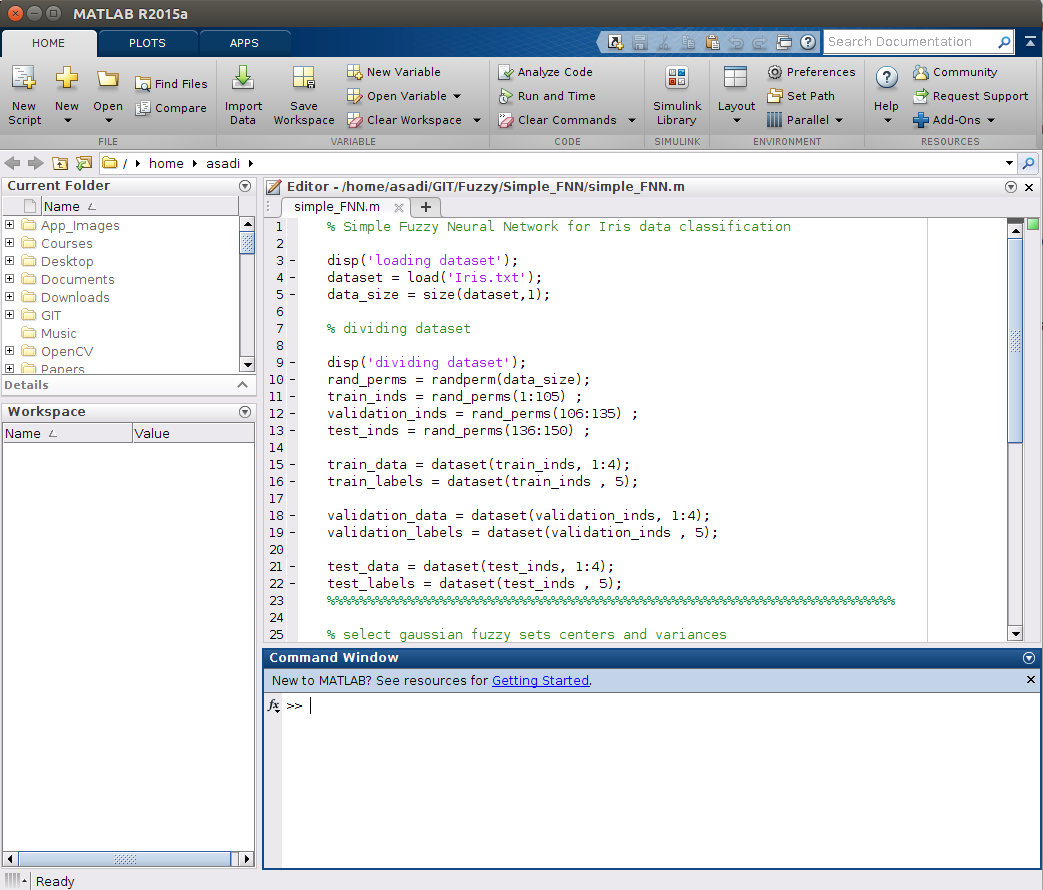
\includegraphics[scale=0.25]{./Imgs/GUI.png}
		\end{figure}
	\end{block}
\end{frame}


\subsection{Basics}


\begin{frame}[fragile]{Primitive data structures}
	\begin{block}{Matrices \& Vectors}
		\begin{itemize}
			\item Almost the most primitive data structures in MATLAB $\rightarrow$ matrices
			\item Defined as bellow:
			\java
				\begin{lstlisting}
	 				>> A = [1 2; 3 4]
	 				A = 		1	2 
	 				     3	4
				\end{lstlisting}
			\item Separate rows by ';' and cols by ',' or ' '
			\item Vectors are special cases of matrices
				\begin{itemize}
					\item [-]\textbf{Row Vector} is an $N*1$ matrix
					\item [-]\textbf{Column Vector} is a $1*M$ matrix
				\end{itemize}
			\item $size(A)$ returns dimensions of matrix $A$
		\end{itemize}
	\end{block}
\end{frame}


\begin{frame}[fragile]{Facilities in Creating Vectors}
	\begin{block}{}
		\begin{itemize}
			\item Creating a vector with equally spaced intervals
			\java
				\begin{lstlisting}
					>> A = 1:0.5:pi
					A =	1.0000	1.5000	2.0000	2.5000	3.0000
				\end{lstlisting}
			\item Creating a vector with $n$ equally spaced intervals
			\java
				\begin{lstlisting}
					>> A = linspace(0, pi, 7)
					A =	0 0.5236	1.0472	1.5708	2.0944	2.6180	3.1416
				\end{lstlisting}
		\end{itemize}
	\end{block}
	\begin{alertblock}{Note}
		\begin{itemize}
			\item [-] MATLAB uses $pi$ to represent $\pi$ and $i$ or $j$ to represent imaginary unit
		\end{itemize}
	\end{alertblock}
\end{frame}



\begin{frame}{Matrices}
	\begin{block}{There is still another useful slide!}
		There exist a list of useful functions being used to create matrices
		\begin{itemize}
			\item[-]$zeros(m,n)$ creates an $m * n$ matrix of all zeros
			\item[-]$ones(m,n)$ creates an $m * n$ matrix of all ones
			\item[-]$eye(m,n)$ creates an $m * n$ identity matrix
			\item[-]$rand(m,n)$ creates an $m * n$ uniformly distributed randoms
			\item[-]$randn(m,n)$ creates an $m * n$ normally distributed randoms
			\item[-]$magic(m)$ creates a square matrix with equal summation of rows, columns and diagonal
			\item[-]$pascal(m)$ creates a square pascal matrix
		\end{itemize}
	\end{block}

\end{frame}

\begin{frame}{Operations}
	\begin{block}{}
		Operations on vectors and matrices are divided into two groups
		\begin{enumerate}
			\item Matrix Operations \\
			Operands of these kind of operations are matrices as whole. 
			\item Array Operations \\
			Operands of these kind of operations are elements of matrices. These kind of operations are being applied to matrices, element by element. 
		\end{enumerate}
	\end{block}
\end{frame}

\begin{frame}{Operations}
	\begin{block}{Matrix Operations}
		\begin{itemize}
			\item [-] $+ \rightarrow $ summation 
			\item [-] $- \rightarrow $ subtraction
			\item [-] $* \rightarrow $ multiplication
			\item [-] $/ \rightarrow $ division  
			\item [-] $\setminus \rightarrow $ left division($ A\setminus B = INV(A) * B$)
			\item [-] $\hat{} \rightarrow $ exponentiation  
		\end{itemize}
	\end{block}
	\begin{block}{Array Operations}
		\begin{itemize}
			\item [-] $.' \rightarrow $ array transpose
			\item [-] $.\hat{} \rightarrow $ array power
			\item [-] $.* \rightarrow $ array multiplication
			\item [-] $./ \rightarrow $ array division  
		\end{itemize}
	\end{block}
\end{frame}

\begin{frame}[fragile]{Reading values of a particle matrix}
	\begin{block}{}
		\begin{itemize}
			\item get value of cell on row 1, col 3 of matrix $A$
			\java
				\begin{lstlisting}
					>> A(1,2)
				\end{lstlisting}
			\item get value of cells on row 2, from col 2 to col 5 of matrix $A$
			\java
				\begin{lstlisting}
					>> A(3,2:5)
				\end{lstlisting}
			\item get value of cells from row 3 to row 6 on col 3 of matrix $A$
			\java
				\begin{lstlisting}
					>> A(3:6,3)
				\end{lstlisting}
			\item get value of cells from row 1 to row 3, from col 2 to row 4 of matrix $A$
			\java
				\begin{lstlisting}
					>> A(1:3,2:4)
				\end{lstlisting}
		\end{itemize}
	\end{block}
\end{frame}

\begin{frame}[fragile]{Reading values of a particle matrix}
	\begin{block}{}
		\begin{itemize}
			\item get value of all cells on row 3 of matrix $A$
			\java
				\begin{lstlisting}
					>> A(3,:)
				\end{lstlisting}
			\item get value of all cells on col 2 of matrix $A$
			\java
				\begin{lstlisting}
					>> A(:,2)
				\end{lstlisting}
			\item get value of all cells of matrix $A$
			\java
				\begin{lstlisting}
					>> A(:,:)
				\end{lstlisting}
		\end{itemize}
	\end{block}
\end{frame}

%parâmetros: linguagem (shell, java, matlab, python, c, php) e arquivo

%\includecode[shell]{codigos/ola.sh}
%
%\includecode[matlab]{codigos/matlab.m}

%ou
% invocar os comandos \ansic, \java, \shell e colocar o código no próprio slide


%\begin{frame}[fragile]{Codigo em C e Java}
%
%\includecode[ansic]{codigos/ola.c}	
%
%\ansic
%	\begin{lstlisting}
%	 int main(void){
%	    printf("Ola mundo\n");
%	    return 0;
%	 }
%	\end{lstlisting}
%\java
%	\begin{lstlisting}
%	 public static voi main(String args[]){
%	    System.out.println("Ola mundo");
%	 }
%	\end{lstlisting}	
%	
%\end{frame}
%
%




\end{document}